% A play of Cops and Robbers on a periodic temporal graph.
% Footprint C_4 (a top-left, b top-right, c bottom-right, d bottom-left), period 2:
%   t even -- the edge da is off;  t odd -- the edge ab is off.
% Cop starts at b, robber at d. The cop catches him in two moves, because at t=0
% the robber's only way out of d is da, which is switched off.
% Verified by exhaustive search. Styles follow JEn2026-01.
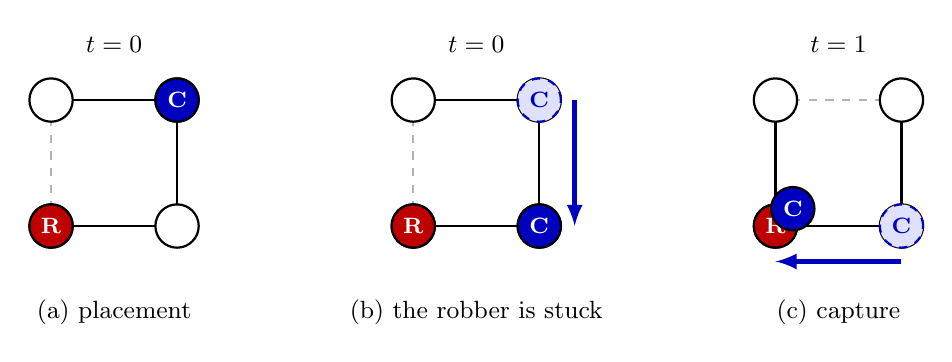
\begin{tikzpicture}[>=latex,
  vertex/.style={circle,draw,thick,fill=white,minimum size=5.5mm,inner sep=0pt},
  cop/.style={vertex,fill=blue!75!black,text=white,font=\bfseries\footnotesize},
  robber/.style={vertex,fill=red!75!black,text=white,font=\bfseries\footnotesize},
  ghostcop/.style={vertex,draw=blue!75!black,dashed,fill=blue!12,text=blue!75!black,font=\bfseries\footnotesize},
  cmove/.style={->,line width=1.6pt,blue!75!black},
  off/.style={dashed,gray!60,thick},
  lab/.style={font=\small},
  tlab/.style={font=\small\itshape},
  square/.pic={
    \foreach \p in {(-0.8,0.8),(0.8,0.8),(0.8,-0.8),(-0.8,-0.8)}
      \node[vertex] at \p {};
  }]

% ---- (a) placement, t = 0 : da is off ----
\begin{scope}[xshift=0cm]
  \draw[thick] (-0.8,0.8)--(0.8,0.8) (0.8,0.8)--(0.8,-0.8) (0.8,-0.8)--(-0.8,-0.8);
  \draw[off]   (-0.8,-0.8)--(-0.8,0.8);
  \pic {square};
  \node[cop]    at (0.8,0.8)   {C};
  \node[robber] at (-0.8,-0.8) {R};
  \node[tlab] at (0,1.5) {$t = 0$};
  \node[lab]  at (0,-1.9) {(a) placement};
\end{scope}

% ---- (b) cop moves b -> c, robber has no move ----
\begin{scope}[xshift=4.6cm]
  \draw[thick] (-0.8,0.8)--(0.8,0.8) (0.8,0.8)--(0.8,-0.8) (0.8,-0.8)--(-0.8,-0.8);
  \draw[off]   (-0.8,-0.8)--(-0.8,0.8);
  \pic {square};
  \node[ghostcop] at (0.8,0.8)   {C};
  \node[cop]      at (0.8,-0.8)  {C};
  \node[robber]   at (-0.8,-0.8) {R};
  \draw[cmove] (1.25,0.8) -- (1.25,-0.8);
  \node[tlab] at (0,1.5) {$t = 0$};
  \node[lab]  at (0,-1.9) {(b) the robber is stuck};
\end{scope}

% ---- (c) t = 1 : ab is off, da is back; cop moves c -> d ----
\begin{scope}[xshift=9.2cm]
  \draw[thick] (0.8,0.8)--(0.8,-0.8) (0.8,-0.8)--(-0.8,-0.8) (-0.8,-0.8)--(-0.8,0.8);
  \draw[off]   (-0.8,0.8)--(0.8,0.8);
  \pic {square};
  \node[ghostcop] at (0.8,-0.8) {C};
  \node[robber]   at (-0.8,-0.8) {R};
  \node[cop]      at (-0.58,-0.58) {C};
  \draw[cmove] (0.8,-1.25) -- (-0.8,-1.25);
  \node[tlab] at (0,1.5) {$t = 1$};
  \node[lab]  at (0,-1.9) {(c) capture};
\end{scope}
\end{tikzpicture}
